% GNUPLOT: LaTeX picture with Postscript
\documentclass{minimal}
% Set font size
\makeatletter
\def\@ptsize{1}
\InputIfFileExists{size11.clo}{}{%
   \GenericError{(gnuplot) \space\space\space\@spaces}{%
      Gnuplot Error: File `size11.clo' not found! Could not set font size%
   }{See the gnuplot documentation for explanation.%
   }{For using a font size a file `size<fontsize>.clo' has to exist.
        Falling back ^^Jto default fontsize 10pt.}%
  \def\@ptsize{0}
  \input{size10.clo}%
}%
\makeatother
% Load packages
\usepackage{graphicx}
\usepackage{color}
\makeatletter
% Select an appropriate default driver (from TeXLive graphics.cfg)
\begingroup
  \chardef\x=0 %
  % check pdfTeX
  \@ifundefined{pdfoutput}{}{%
    \ifcase\pdfoutput
    \else
      \chardef\x=1 %
    \fi
  }%
  % check VTeX
  \@ifundefined{OpMode}{}{%
    \chardef\x=2 %
  }%
\expandafter\endgroup
\ifcase\x
  % default case
  \PassOptionsToPackage{dvips}{geometry}
\or
  % pdfTeX is running in pdf mode
  \PassOptionsToPackage{pdftex}{geometry}
\else
  % VTeX is running
  \PassOptionsToPackage{vtex}{geometry}
\fi
\makeatother
% Set papersize
\usepackage[papersize={360.00bp,252.00bp},text={360.00bp,252.00bp}]{geometry}
% No page numbers and no paragraph indentation
\pagestyle{empty}
\setlength{\parindent}{0bp}%
% Load configuration file
\InputIfFileExists{gnuplot.cfg}{%
  \typeout{Using configuration file gnuplot.cfg}%
}{%
 \typeout{No configuration file gnuplot.cfg found.}%
}%
%
\begin{document}
\begingroup
  \makeatletter
  \providecommand\color[2][]{%
    \GenericError{(gnuplot) \space\space\space\@spaces}{%
      Package color not loaded in conjunction with
      terminal option `colourtext'%
    }{See the gnuplot documentation for explanation.%
    }{Either use 'blacktext' in gnuplot or load the package
      color.sty in LaTeX.}%
    \renewcommand\color[2][]{}%
  }%
  \providecommand\includegraphics[2][]{%
    \GenericError{(gnuplot) \space\space\space\@spaces}{%
      Package graphicx or graphics not loaded%
    }{See the gnuplot documentation for explanation.%
    }{The gnuplot epslatex terminal needs graphicx.sty or graphics.sty.}%
    \renewcommand\includegraphics[2][]{}%
  }%
  \providecommand\rotatebox[2]{#2}%
  \@ifundefined{ifGPcolor}{%
    \newif\ifGPcolor
    \GPcolorfalse
  }{}%
  \@ifundefined{ifGPblacktext}{%
    \newif\ifGPblacktext
    \GPblacktexttrue
  }{}%
  % define a \g@addto@macro without @ in the name:
  \let\gplgaddtomacro\g@addto@macro
  % define empty templates for all commands taking text:
  \gdef\gplbacktext{}%
  \gdef\gplfronttext{}%
  \makeatother
  \ifGPblacktext
    % no textcolor at all
    \def\colorrgb#1{}%
    \def\colorgray#1{}%
  \else
    % gray or color?
    \ifGPcolor
      \def\colorrgb#1{\color[rgb]{#1}}%
      \def\colorgray#1{\color[gray]{#1}}%
      \expandafter\def\csname LTw\endcsname{\color{white}}%
      \expandafter\def\csname LTb\endcsname{\color{black}}%
      \expandafter\def\csname LTa\endcsname{\color{black}}%
      \expandafter\def\csname LT0\endcsname{\color[rgb]{1,0,0}}%
      \expandafter\def\csname LT1\endcsname{\color[rgb]{0,1,0}}%
      \expandafter\def\csname LT2\endcsname{\color[rgb]{0,0,1}}%
      \expandafter\def\csname LT3\endcsname{\color[rgb]{1,0,1}}%
      \expandafter\def\csname LT4\endcsname{\color[rgb]{0,1,1}}%
      \expandafter\def\csname LT5\endcsname{\color[rgb]{1,1,0}}%
      \expandafter\def\csname LT6\endcsname{\color[rgb]{0,0,0}}%
      \expandafter\def\csname LT7\endcsname{\color[rgb]{1,0.3,0}}%
      \expandafter\def\csname LT8\endcsname{\color[rgb]{0.5,0.5,0.5}}%
    \else
      % gray
      \def\colorrgb#1{\color{black}}%
      \def\colorgray#1{\color[gray]{#1}}%
      \expandafter\def\csname LTw\endcsname{\color{white}}%
      \expandafter\def\csname LTb\endcsname{\color{black}}%
      \expandafter\def\csname LTa\endcsname{\color{black}}%
      \expandafter\def\csname LT0\endcsname{\color{black}}%
      \expandafter\def\csname LT1\endcsname{\color{black}}%
      \expandafter\def\csname LT2\endcsname{\color{black}}%
      \expandafter\def\csname LT3\endcsname{\color{black}}%
      \expandafter\def\csname LT4\endcsname{\color{black}}%
      \expandafter\def\csname LT5\endcsname{\color{black}}%
      \expandafter\def\csname LT6\endcsname{\color{black}}%
      \expandafter\def\csname LT7\endcsname{\color{black}}%
      \expandafter\def\csname LT8\endcsname{\color{black}}%
    \fi
  \fi
  \setlength{\unitlength}{0.0500bp}%
  \begin{picture}(7200.00,5040.00)%
    \gplgaddtomacro\gplbacktext{%
      \csname LTb\endcsname%
      \put(3566,1007){\makebox(0,0){\strut{}Note that overlapping transparent circles produce a darker area}}%
      \put(3566,3812){\makebox(0,0){\strut{}}}%
    }%
    \gplgaddtomacro\gplfronttext{%
    }%
    \gplgaddtomacro\gplbacktext{%
      \csname LTb\endcsname%
      \put(3566,3999){\makebox(0,0){\strut{}Sources of energy production, plotted for each continent}}%
    }%
    \gplgaddtomacro\gplfronttext{%
      \csname LTb\endcsname%
      \put(1463,1720){\makebox(0,0){\strut{}Coal}}%
      \csname LTb\endcsname%
      \put(1083,1501){\makebox(0,0){\strut{}Oil}}%
      \csname LTb\endcsname%
      \put(702,1720){\makebox(0,0){\strut{}Gas}}%
      \csname LTb\endcsname%
      \put(702,2159){\makebox(0,0){\strut{}Nuclear}}%
      \csname LTb\endcsname%
      \put(1083,2378){\makebox(0,0){\strut{}Hydroelectric}}%
      \csname LTb\endcsname%
      \put(1463,2159){\makebox(0,0){\strut{}Renewable}}%
    }%
    \gplgaddtomacro\gplbacktext{%
      \put(1448,440){\makebox(0,0)[r]{\strut{}-1}}%
      \put(1448,1003){\makebox(0,0)[r]{\strut{}-0.5}}%
      \put(1448,1565){\makebox(0,0)[r]{\strut{} 0}}%
      \put(1448,2128){\makebox(0,0)[r]{\strut{} 0.5}}%
      \put(1448,2691){\makebox(0,0)[r]{\strut{} 1}}%
      \put(1448,3254){\makebox(0,0)[r]{\strut{} 1.5}}%
      \put(1448,3816){\makebox(0,0)[r]{\strut{} 2}}%
      \put(1448,4379){\makebox(0,0)[r]{\strut{} 2.5}}%
      \put(1580,220){\makebox(0,0){\strut{}-2.5}}%
      \put(2143,220){\makebox(0,0){\strut{}-2}}%
      \put(2705,220){\makebox(0,0){\strut{}-1.5}}%
      \put(3268,220){\makebox(0,0){\strut{}-1}}%
      \put(3831,220){\makebox(0,0){\strut{}-0.5}}%
      \put(4393,220){\makebox(0,0){\strut{} 0}}%
      \put(4956,220){\makebox(0,0){\strut{} 0.5}}%
      \put(5518,220){\makebox(0,0){\strut{} 1}}%
      \put(6081,220){\makebox(0,0){\strut{} 1.5}}%
      \put(3830,4709){\makebox(0,0){\strut{}Trace of unconstrained optimization with trust-region method}}%
    }%
    \gplgaddtomacro\gplfronttext{%
    }%
    \gplgaddtomacro\gplbacktext{%
      \csname LTb\endcsname%
      \put(3566,4709){\makebox(0,0){\strut{}Lena's key points}}%
    }%
    \gplgaddtomacro\gplfronttext{%
    }%
    \gplgaddtomacro\gplbacktext{%
      \csname LTb\endcsname%
      \put(1729,440){\makebox(0,0)[r]{\strut{}-100}}%
      \put(1729,834){\makebox(0,0)[r]{\strut{}-80}}%
      \put(1729,1228){\makebox(0,0)[r]{\strut{}-60}}%
      \put(1729,1622){\makebox(0,0)[r]{\strut{}-40}}%
      \put(1729,2016){\makebox(0,0)[r]{\strut{}-20}}%
      \put(1729,2410){\makebox(0,0)[r]{\strut{} 0}}%
      \put(1729,2803){\makebox(0,0)[r]{\strut{} 20}}%
      \put(1729,3197){\makebox(0,0)[r]{\strut{} 40}}%
      \put(1729,3591){\makebox(0,0)[r]{\strut{} 60}}%
      \put(1729,3985){\makebox(0,0)[r]{\strut{} 80}}%
      \put(1729,4379){\makebox(0,0)[r]{\strut{} 100}}%
      \put(1861,220){\makebox(0,0){\strut{}-100}}%
      \put(2255,220){\makebox(0,0){\strut{}-80}}%
      \put(2649,220){\makebox(0,0){\strut{}-60}}%
      \put(3043,220){\makebox(0,0){\strut{}-40}}%
      \put(3437,220){\makebox(0,0){\strut{}-20}}%
      \put(3831,220){\makebox(0,0){\strut{} 0}}%
      \put(4224,220){\makebox(0,0){\strut{} 20}}%
      \put(4618,220){\makebox(0,0){\strut{} 40}}%
      \put(5012,220){\makebox(0,0){\strut{} 60}}%
      \put(5406,220){\makebox(0,0){\strut{} 80}}%
      \put(5800,220){\makebox(0,0){\strut{} 100}}%
      \put(3830,4709){\makebox(0,0){\strut{}Delaunay triangulation of Hemisphere points, some empty circles in red}}%
    }%
    \gplgaddtomacro\gplfronttext{%
    }%
    \gplbacktext
    \put(0,0){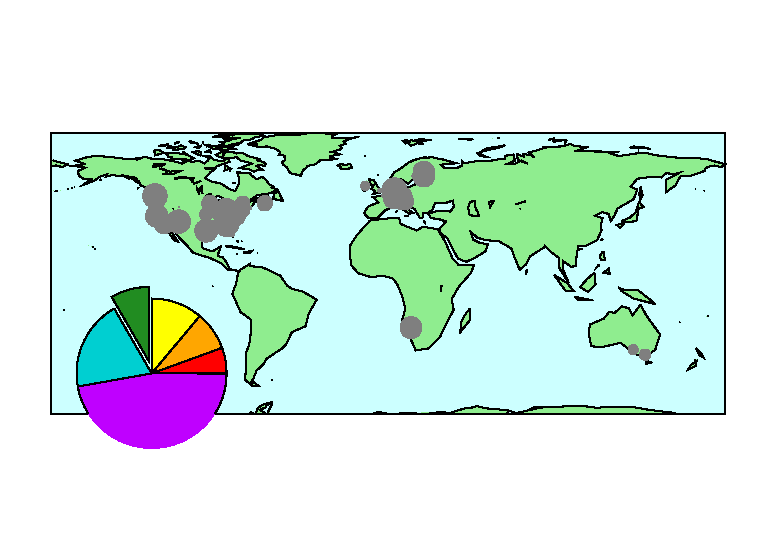
\includegraphics{circles-inc}}%
    \gplfronttext
  \end{picture}%
\endgroup
\end{document}
